\section{Theoretical Background}
\subsection{Phase accumulator}

Phase Accumulator là một thanh ghi (register) n-bit chạy modulo $ 2^{n} $, mỗi chu kỳ xung clock nó sẽ cộng thêm một giá trị cố định $M$ (Frequency Control Word: gọi tắt là FCW hay tunning word) là một số (thường là số nguyên) được đưa vào bộ tích lũy pha để điều khiển tốc độ tăng pha, từ đó quyết định tần số sóng đầu ra.

$ FCW = M $ là giá trị “\textit{nhảy pha}” (phase step) mỗi chu kỳ. Nếu FCW lớn, pha tăng nhanh, tần số sóng cao. Nếu FCW nhỏ, pha tăng chậm, tần số thấp.
 
\textbf{Cách hoạt động:} Mỗi khi có một xung clock (nhịp đồng hồ), bộ tích lũy pha sẽ cộng thêm một giá trị cố định vào giá trị hiện tại của nó

$ \Leftarrow $ Kết quả tích lũy chính là “\textit{pha}” (phase) hiện tại, tăng đều đặn từ $ 0 \leftarrow 2^{n} - 1 $ rồi quay vòng về $ 0 $, xây dựng nên một “\textit{bánh xe pha}” (phase wheel) tuyến tính như hình \ref{fig: banh xe pha}.

\begin{figure}[H]
	\centering
	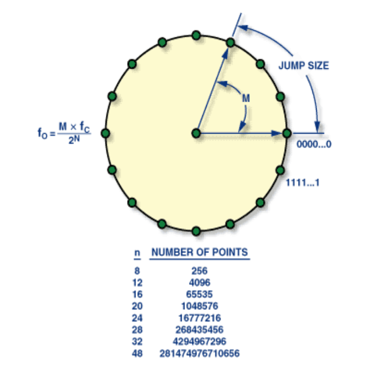
\includegraphics[width=.6\linewidth]{./my-chapters/my-images/Gen_wave/hinh1.png}
	\caption{Bánh xe pha.}
	\label{fig: banh xe pha}
\end{figure}

Giá trị này tăng dần, giống như một đường dốc (ramp). Khi nó đạt đến giá trị tối đa thì nó sẽ "tràn" (overflow) và quay lại 0 giống như kim đồng hồ quay hết một vòng rồi trở lại vị trí ban đầu.

$ \Leftarrow $ Ta còn gọi đây là hiện tượng wrap-around. 

Tốc độ tăng của nó quyết định tần số sóng đầu ra theo công thức:
\[ f_{out} = \dfrac{M}{2^{n}} f_{clk} \]

Trong đó,

\begin{itemize}[label=-]
	\item $ FCW = M $ là giá trị “\textit{nhảy pha}” (phase step) mỗi chu kỳ. Nếu FCW lớn, pha tăng nhanh, tần số sóng cao. Nếu FCW nhỏ, pha tăng chậm, tần số thấp.
	\item n: Số bit của bộ tích lũy pha.
	\item $ f_{clk} $: Tần số điều khiển phase accumulator.
	\item $ f_{out} $: Tần số đầu ra mong muốn.
\end{itemize}

\subsection{Ý tưởng tạo các loại sóng}

Trước tiên, đối với các sóng dạng phức tạp như sin hay ECG thì ta tạo sóng bằng cách cộng dồn pha và ánh xạ pha này sang biên độ sóng thông qua \textbf{bảng tra (LUT)}.

\subsubsection{Sóng Sin}

Ý tưởng thực hiện: Tổng có $ 1024 $ mẫu tức là phải lưu đầy đủ từ $ 0^{o} \leftarrow 360^{o} $ cho cả 1 chu kỳ sóng sin. Nhưng làm vậy sẽ tốn gấp 4 lần dung lượng ROM $ \leftarrow $ Nếu chỉ cần $ \dfrac{1}{4} $ chu kỳ, nghĩa là lưu từ $ 0^{o} \leftarrow 90^{o} $.

Đầu tiên, ta dùng bit MSB để phân biệt 2 vùng sin dương ($ 0^{o} \leftarrow 180^{o} $ ở 2 phần tư đầu của chu kỳ và vùng sin âm ($ 180^{o} \leftarrow 360^{o} $) ở 2 phần tư còn lại. Tiếp theo, tại mỗi vùng, ta dùng bit[MSB-1] làm mốc đổi xứng để cho ta biết khi nào cần thực hiện đảo địa chỉvà thu được nửa sóng sin hoàn chỉnh.

Với nửa chu kỳ dương đầu tiên của sóng sin, ta chọn phase step tùy thuộc vào tần số đầu ra mong muốn. Bộ Phase accumulator sẽ tích lũy và tăng dần địa chỉ ở phần tư đầu tiên theo $ \dfrac{1}{4} $ mẫu đã lưu khi bit[MSB-1] = 0. Nếu bit[MSB-1]=1 thì thực hiện đảo (mirror) bằng cách lấy giá trị Maxium - địa chỉ của phần tư đầu tiên hoặc ta thực hiện  phép NOT địa chỉ của phần tư đầu tiên. Ta thu được phần thứ hai và hoàn chỉnh được nửa chu kỳ dương của sóng sin.

Với nửa chu kỳ âm, ta cần thực hiện lấy bù 2 để chuyển vùng từ dương sang âm dựa vào bit MSB = 1. Sau đó, mirror để thu được phần tư thứ ba của sóng sin. Cuối cùng, phần tư cuối sẽ mirror lại phần tư thứ ba.

Tóm lại, bit MSB để quyết định vùng dương hoặc âm, bit[MSB-1] để quyết định lấy đảo (mirror) hay không.

Kết quả thu được:

\begin{figure}[H]
	\centering
	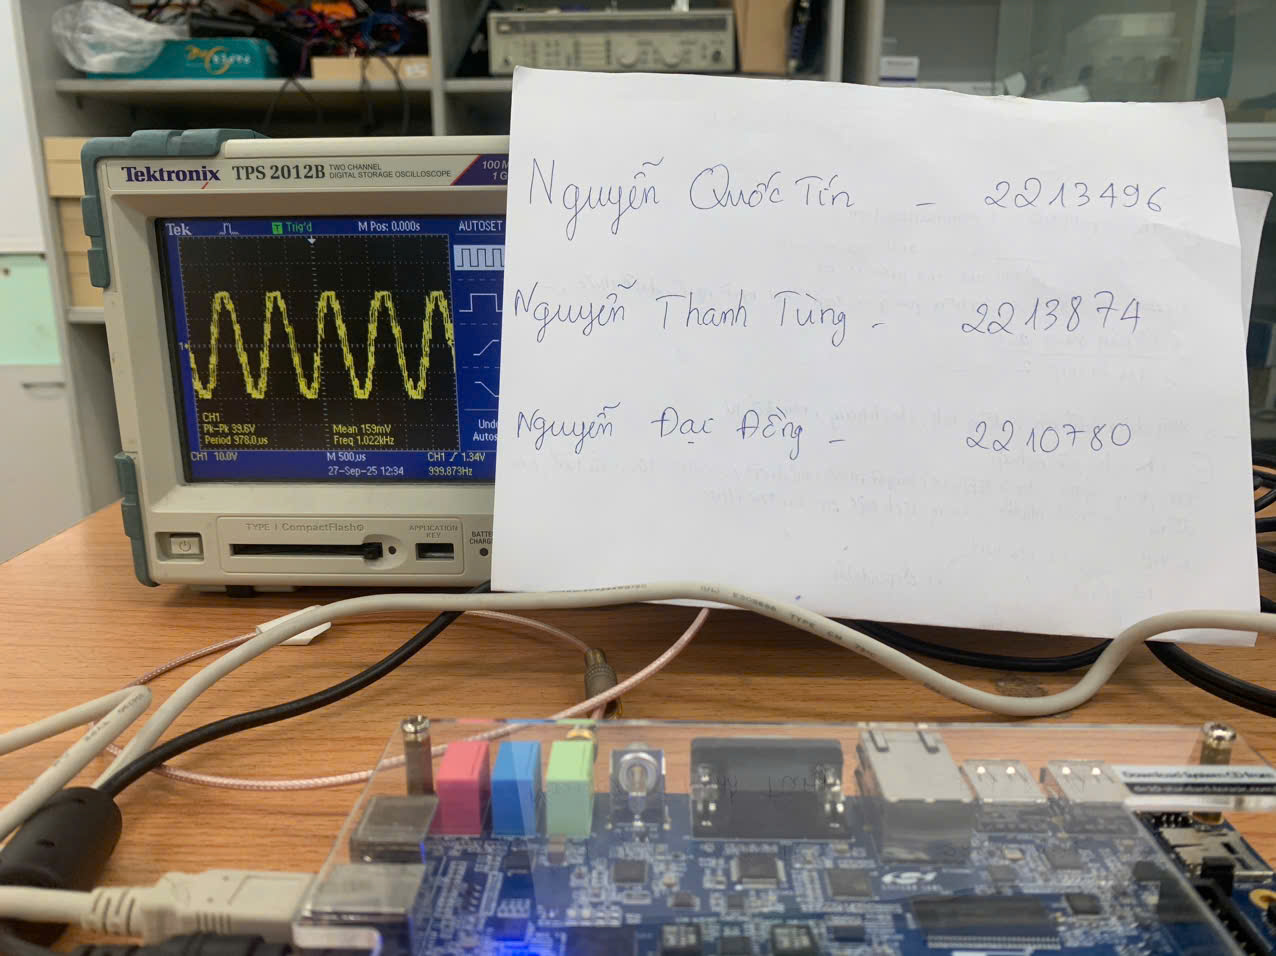
\includegraphics[width=\linewidth]{./my-chapters/my-images/Gen_wave/hinh2.jpg}
	\caption{Sóng Sin khi đổ KIT.}
	\label{f: sin wave}
\end{figure}

\subsubsection{Sóng ECG}

Với sóng ECG khá phức tạp, nên nhóm sẽ sử dụng file HEX chức năng là làm LUT với 1024 mẫu. Tương tự, Phase accumulator sẽ tích lũy pha và tăng dần địa chỉ với mỗi địa chỉ chứa một giá trị biên độ của ECG. Nhờ đó, ROM lần lượt xuất ra từng mẫu ECG. Thực hiện ghép các mẫu liên tiếp theo thời gian sẽ thành sóng ECG hoàn chỉnh. Kêt quả thu được:

\begin{figure}[H]
	\centering
	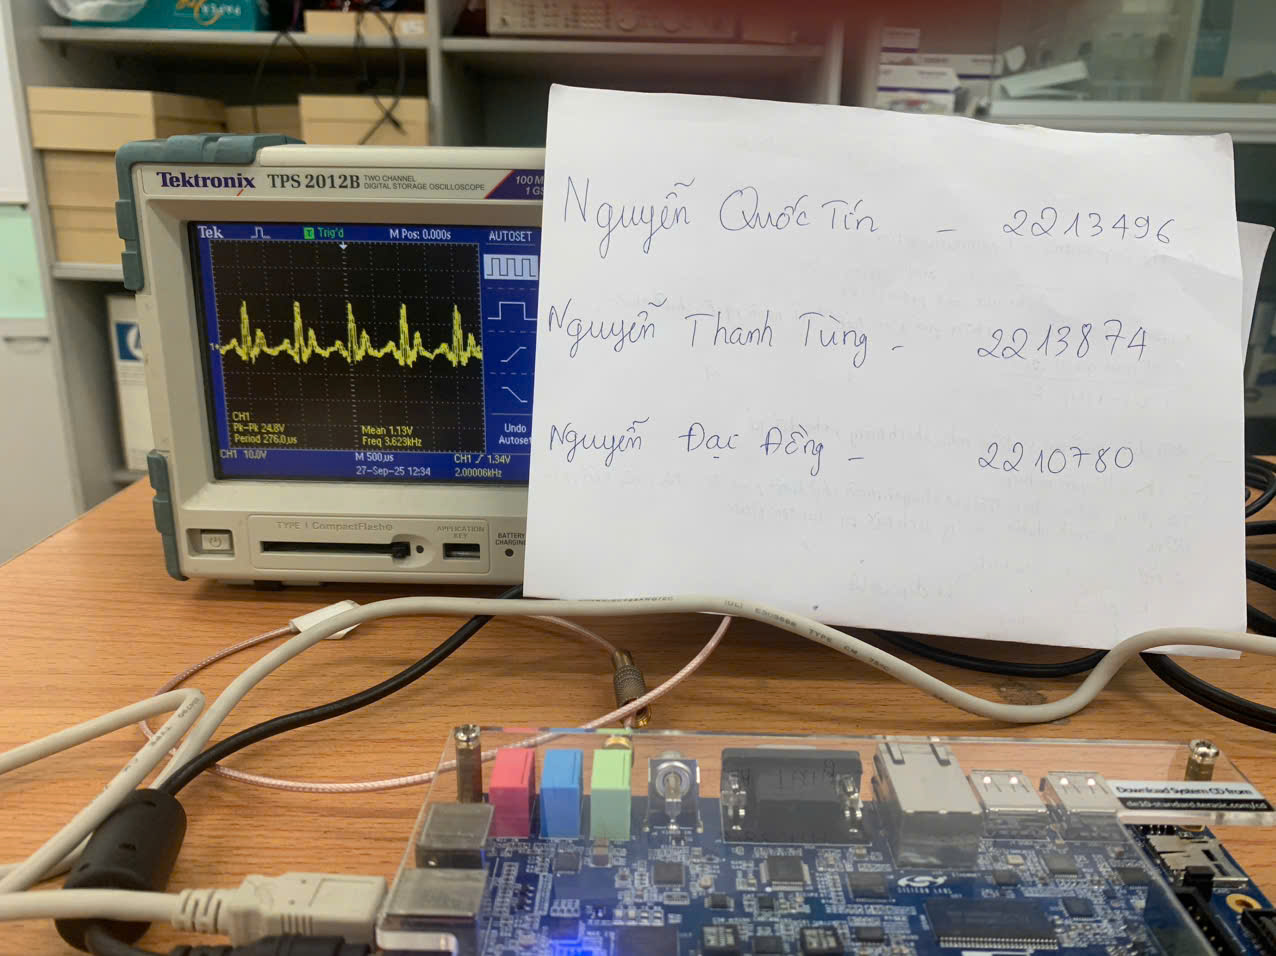
\includegraphics[width=\linewidth]{./my-chapters/my-images/Gen_wave/hinh3.jpg}
	\caption{Sóng ECG khi đổ KIT.}
	\label{f: ecg wave}
\end{figure}

\subsubsection{Sóng vuông}

Đối với sóng vuông đơn giản, ta thực hiện nó bằng logic bằng không cần dùng tới LUT. Cụ thể:

Bộ Phase accumulator đóng vai trò làm “thước đo” thời gian trong một chu kỳ sóng. Một chu kỳ sóng vuông có hai mức: HIGH (24'h0FFF00) và LOW (24'h0). Sóng được xác định bằng cách so sánh pha đã tích lũy được với các ngưỡng (threshold).

Xác định những giá trị duty cycle mong muốn là bao nhiêu. Từ đó, xác định giá trị ngưỡng để xác định HIGH và LOW. Ví dụ: duty cycle = 90\% của 1024 giá trị thì cần đếm $ 10’d102 $ để thực hiện mức LOW trước và ta chọn điểm này làm ngưỡng. Khi vượt ngưỡng thì đảo lại HIGH . Tương tự cho các giá trị duty cycle khác.

Một vài duty cycle đặc biệt như 50\% thì ta có thể lợi dụng tính đối xứng dựa vào bit MSB. Đếm đủ một nửa MSB = 0 thì thực hiện đảo ở MSB = 1. Hay duty cycle = 75\%, 25\% thì ta thực hiện OR 2 bit MSB.

\subsubsection{Sóng răng cưa}

Ta thực hiện tích lũy pha như mọi sóng khác, lợi dụng hiện tượng wrap-around để tích lũy pha dần (đường ramp tuyến tính) và khi tràn sẽ lập tức quay về 0. Kết quả thu được:

\begin{figure}[H]
	\centering
	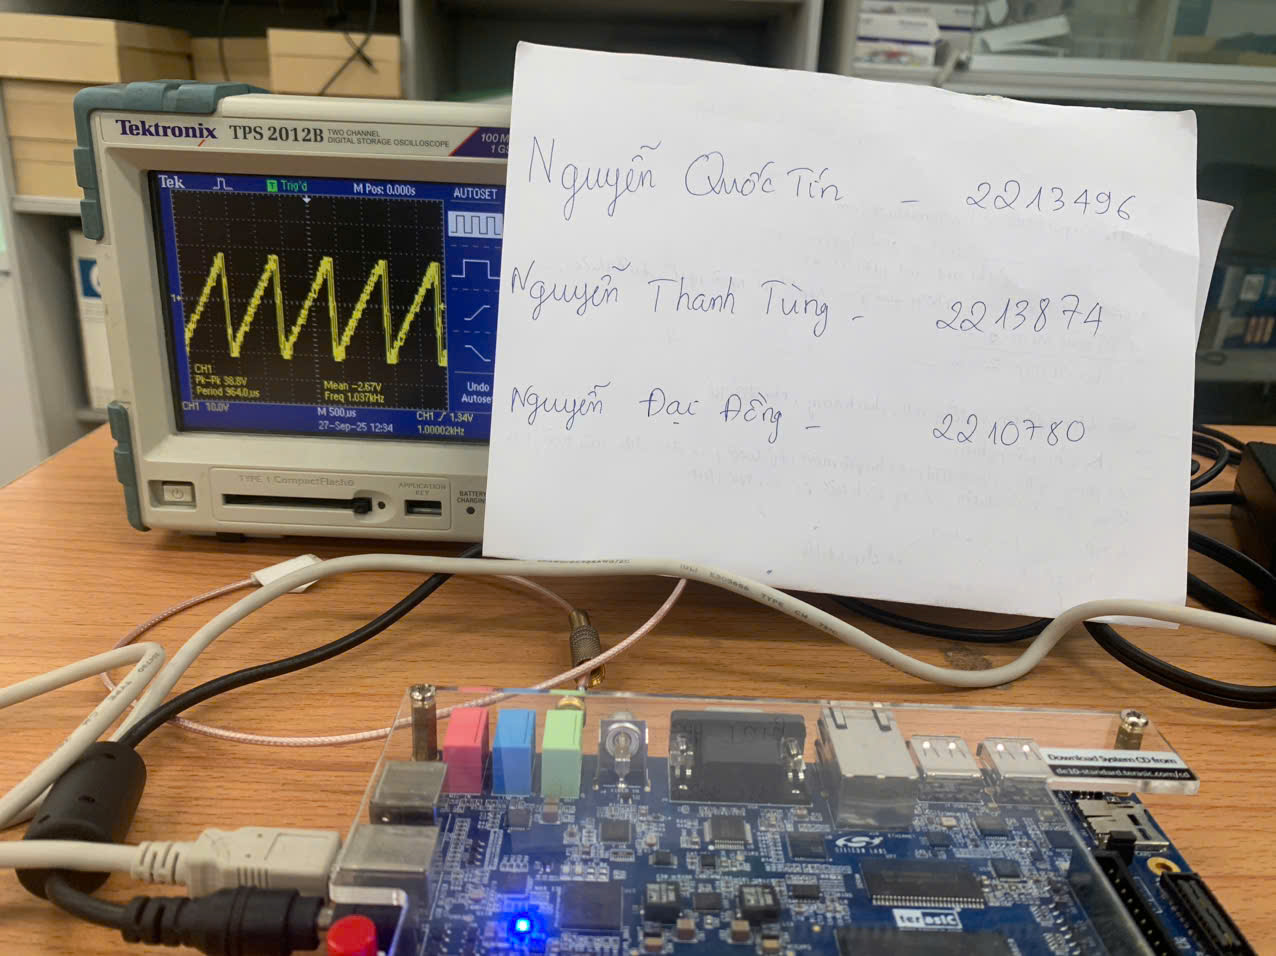
\includegraphics[width=\linewidth]{./my-chapters/my-images/Gen_wave/hinh4.jpg}
	\caption{Sóng Răng cưa.}
	\label{f: sawtooth_wave}
\end{figure}

\subsubsection{Sóng tam giác}

Được tạo dựa vào sóng răng cưa với 2 đường ramp tăng tuyến tính ở nửa đầu và giảm tuyến tính ở nửa sau. Thực hiện bằng cách tích lũy pha tạo đường ramp tuyến tính như sóng răng cưa. Sau đó, lợi dụng tính đối xứng dựa vào bit MSB để đảo đường ramp ở nửa phần sau hoặc lấy giá trị Maximum – giá trị tích lũy dần ở nửa đường ramp thứ nhất. Kết quả thu được:

\begin{figure}[H]
	\centering
	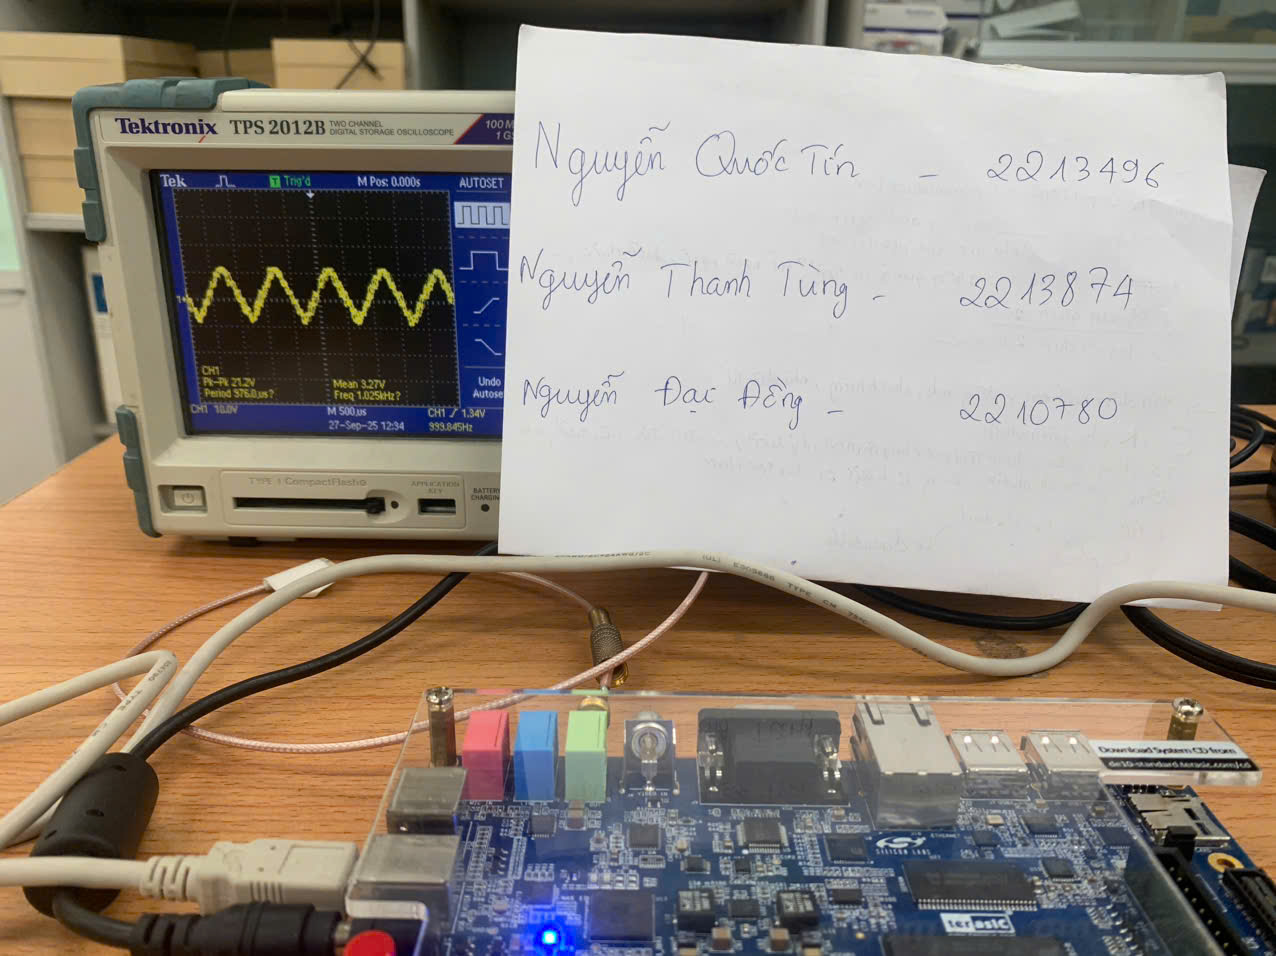
\includegraphics[width=\linewidth]{./my-chapters/my-images/Gen_wave/hinh5.jpg}
	\caption{Sóng tam giác.}
	\label{f: triangle_wave}
\end{figure}